% answers.tex —— 2005 年·普通高等学校招生考试·福建卷·文科 · 参考答案与详细解析片段
% 由 tools/generate_projects.py 依来源总账自 2005/2005_数学真题_福建文科_试题.md + 2005/2005_数学真题_福建文科_解析正文.md + 2005/2005_数学真题_福建文科_答案要点.md 生成，勿手改（改源 MD 后重跑）

\begin{answer}
\gksolhead{1}{}

\textbf{题目}：

已知集合 $P = \{x \mid |x - 1| \leqslant 1, x \in \mathbf{R}\}$，集合 $Q = \{x \mid x \in \mathbf{N}\}$，则 $P \cap Q$ 等于\mbox{（　　）}

\begin{gkopts}(4)
\task A．$P$
\task B．$Q$
\task C．$\{1, 2\}$
\task D．$\{0, 1, 2\}$
\end{gkopts}

\Needspace{4\baselineskip}
\textbf{解析}

\Needspace{5\baselineskip}
由集合 $P$ 中的绝对值不等式：
\nopagebreak[4]
\[
|x - 1| \leqslant 1 \iff -1 \leqslant x - 1 \leqslant 1 \iff 0 \leqslant x \leqslant 2,
\]
所以 $P = \{x \in \mathbf{R} \mid 0 \leqslant x \leqslant 2\}$．
集合 $Q = \{x \mid x \in \mathbf{N}\}$ 为自然数集，即 $Q = \{0, 1, 2, 3, \dots\}$．
\Needspace{5\baselineskip}
因此：
\nopagebreak[4]
\[
P \cap Q = \{0, 1, 2\}.
\]
故选 D．

\gkanswer{答案：D}

\end{answer}
\begin{answer}
\gksolhead{2}{}

\textbf{题目}：

不等式 $\dfrac{2x - 1}{3x + 1} > 0$ 的解集是\mbox{（　　）}

\begin{gkopts}(1)
\task A．$\left\{x \mathrel{}\middle|\mathrel{} x < -\dfrac{1}{3} \text{ \text{或} } x > \dfrac{1}{2}\right\}$
\task B．$\left\{x \mathrel{}\middle|\mathrel{} -\dfrac{1}{3} < x < \dfrac{1}{2}\right\}$
\task C．$\left\{x \mathrel{}\middle|\mathrel{} x > \dfrac{1}{2}\right\}$
\task D．$\left\{x \mathrel{}\middle|\mathrel{} x > -\dfrac{1}{3}\right\}$
\end{gkopts}

\Needspace{4\baselineskip}
\textbf{解析}

\Needspace{5\baselineskip}
分式不等式 $\dfrac{2x - 1}{3x + 1} > 0$ 等价于二次不等式：
\nopagebreak[4]
\[
(2x - 1)(3x + 1) > 0.
\]
方程 $(2x - 1)(3x + 1) = 0$ 的两根为 $x_1 = -\dfrac{1}{3}$ 与 $x_2 = \dfrac{1}{2}$．
\Needspace{5\baselineskip}
根据二次不等式“大于取两边”，原不等式的解集为：
\nopagebreak[4]
\[
\left\{x \mathrel{}\middle|\mathrel{} x < -\frac{1}{3} \text{ \text{或} } x > \frac{1}{2}\right\}.
\]
故选 A．

\gkanswer{答案：A}

\end{answer}
\begin{answer}
\gksolhead{3}{}

\textbf{题目}：

已知等差数列 $\{a_n\}$ 中，$a_7 + a_9 = 16$，$a_4 = 1$，则 $a_{12}$ 的值是\mbox{（　　）}

\begin{gkopts}(4)
\task A．$15$
\task B．$30$
\task C．$31$
\task D．$64$
\end{gkopts}

\Needspace{4\baselineskip}
\textbf{解析}

设等差数列 $\{a_n\}$ 的公差为 $d$．
\Needspace{5\baselineskip}
由等差数列的性质，下标满足 $7 + 9 = 2 \times 8$，因此：
\nopagebreak[4]
\[
a_7 + a_9 = 2a_8 = 16 \implies a_8 = 8.
\]
\Needspace{5\baselineskip}
又已知 $a_4 = 1$，则：
\nopagebreak[4]
\[
a_8 - a_4 = 4d \implies 8 - 1 = 4d \implies 4d = 7.
\]
\Needspace{5\baselineskip}
所以：
\nopagebreak[4]
\[
a_{12} = a_8 + 4d = 8 + 7 = 15.
\]
故选 A．

\gkanswer{答案：A}

\end{answer}
\begin{answer}
\gksolhead{4}{}

\textbf{题目}：

函数 $y = \cos 2x$ 在下列哪个区间上是减函数\mbox{（　　）}

\begin{gkopts}(1)
\task A．$\left[-\dfrac{\pi}{4}, \dfrac{\pi}{4}\right]$
\task B．$\left[\dfrac{\pi}{4}, \dfrac{3\pi}{4}\right]$
\task C．$\left[0, \dfrac{\pi}{2}\right]$
\task D．$\left[\dfrac{\pi}{2}, \pi\right]$
\end{gkopts}

\Needspace{4\baselineskip}
\textbf{解析}

对于余弦函数 $y = \cos u$，其单调递减区间由 $2k\pi \leqslant u \leqslant 2k\pi + \pi$（$k \in \mathbf{Z}$）给出．
\Needspace{5\baselineskip}
令 $u = 2x$，得：
\nopagebreak[4]
\[
2k\pi \leqslant 2x \leqslant 2k\pi + \pi \iff k\pi \leqslant x \leqslant k\pi + \frac{\pi}{2} \quad (k \in \mathbf{Z}).
\]
取 $k = 0$，得函数 $y = \cos 2x$ 的一个单调递减区间为 $\left[0, \dfrac{\pi}{2}\right]$．
各选项对照可知，C 选项正确．
故选 C．

\gkanswer{答案：C}

\end{answer}
\begin{answer}
\gksolhead{5}{}

\textbf{题目}：

下列结论正确的是\mbox{（　　）}

\begin{gkopts}(1)
\task A．当 $x > 0$ 且 $x \neq 1$ 时，$\lg x + \dfrac{1}{\lg x} \geqslant 2$
\task B．当 $x > 0$ 时，$\sqrt{x} + \dfrac{1}{\sqrt{x}} \geqslant 2$
\task C．当 $x \geqslant 2$ 时，$x + \dfrac{1}{x}$ 的最小值为 $2$
\task D．当 $0 < x \leqslant 2$ 时，$x - \dfrac{1}{x}$ 无最大值
\end{gkopts}

\Needspace{4\baselineskip}
\textbf{解析}

逐项分析：
对于 A 选项：当 $0 < x < 1$ 时，$\lg x < 0$，由基本不等式可知 $\lg x + \dfrac{1}{\lg x} \leqslant -2$，故 A 错误；
对于 B 选项：当 $x > 0$ 时，$\sqrt{x} > 0$，由基本不等式可得 $\sqrt{x} + \dfrac{1}{\sqrt{x}} \geqslant 2\sqrt{\sqrt{x} \cdot \dfrac{1}{\sqrt{x}}} = 2$，当且仅当 $\sqrt{x} = 1$ 即 $x = 1$ 时等号成立，故 B 正确；
对于 C 选项：函数 $y = x + \dfrac{1}{x}$ 在 $[1, +\infty)$ 上单调递增，当 $x \geqslant 2$ 时，最小值为 $2 + \dfrac{1}{2} = \dfrac{5}{2} \neq 2$，故 C 错误；
对于 D 选项：函数 $y = x - \dfrac{1}{x}$ 在 $(0, 2]$ 上是单调递增函数，当 $x = 2$ 时取得最大值 $2 - \dfrac{1}{2} = \dfrac{3}{2}$，故 D 错误．
故选 B．

\gkanswer{答案：B}

\end{answer}
\begin{answer}
\gksolhead{6}{}

\textbf{题目}：

若函数 $f(x) = a^{x-b}$ 的图象如图，其中 $a$、$b$ 为常数，则下列结论正确的是\mbox{（　　）}
\nopagebreak[4]
\begin{center}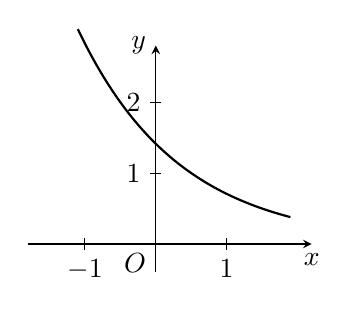
\begin{tikzpicture}[>=stealth, scale=0.9]
  % 坐标轴
  \draw[->] (-1.8, 0) -- (2.2, 0) node[below] {$x$};
  \draw[->] (0, -0.4) -- (0, 2.8) node[left] {$y$};
  \node[below left] at (0, 0) {$O$};

  % 刻度
  \draw (-1, 0.08) -- (-1, -0.08) node[below] {$-1$};
  \draw (1, 0.08) -- (1, -0.08) node[below] {$1$};
  \draw (0.08, 1) -- (-0.08, 1) node[left] {$1$};
  \draw (0.08, 2) -- (-0.08, 2) node[left] {$2$};

  % 指数函数曲线 (例如 a=0.5, b=0.5 即 y = 0.5^(x - 0.5))
  \draw[thick, domain=-1.1:1.9, samples=50] plot (\x, {pow(0.5, \x - 0.5)});
\end{tikzpicture}
\end{center}
\nopagebreak[4]
\begin{gkopts}(2)
\task A．$a > 1, b < 0$
\task B．$a > 1, b > 0$
\task C．$0 < a < 1, b > 0$
\task D．$0 < a < 1, b < 0$
\end{gkopts}

\Needspace{4\baselineskip}
\textbf{解析}

由函数图象可知：
第一，曲线从左向右下降，函数在定义域 $\mathbf{R}$ 上单调递减，因此底数满足 $0 < a < 1$；
\Needspace{5\baselineskip}
第二，当 $x = 0$ 时，图象与 $y$ 轴的交点在点 $(0, 1)$ 的上方，即：
\nopagebreak[4]
\[
f(0) = a^{-b} > 1.
\]
\Needspace{5\baselineskip}
因为 $0 < a < 1$，由指数函数单调性可得：
\nopagebreak[4]
\[
-b < 0 \implies b > 0.
\]
（亦可由图象与直线 $y = 1$ 的交点横坐标判定：令 $a^{x-b} = 1 \implies x - b = 0 \implies x = b$；从图中可见该交点的横坐标在原点右侧，即 $b > 0$）．
综上所述，$0 < a < 1$ 且 $b > 0$．
故选 C．

\gkanswer{答案：C}

\end{answer}
\begin{answer}
\gksolhead{7}{}

\textbf{题目}：

已知直线 $m$、$n$ 与平面 $\alpha, \beta$，给出下列三个命题：
① 若 $m \parallel \alpha, n \parallel \alpha$，则 $m \parallel n$；
② 若 $m \parallel \alpha, n \perp \alpha$，则 $n \perp m$；
③ 若 $m \perp \alpha, m \parallel \beta$，则 $\alpha \perp \beta$．
其中真命题的个数是\mbox{（　　）}

\begin{gkopts}(4)
\task A．$0$
\task B．$1$
\task C．$2$
\task D．$3$
\end{gkopts}

\Needspace{4\baselineskip}
\textbf{解析}

逐一分析三个命题：
① 若 $m \parallel \alpha, n \parallel \alpha$，则直线 $m$ 与 $n$ 可以平行、相交或异面，故 ① 为假命题；
② 若 $m \parallel \alpha$，则存在平面 $\gamma$ 经过直线 $m$，设 $\gamma \cap \alpha = l$，则由线面平行的性质定理可知 $m \parallel l$．又因为 $n \perp \alpha$，且 $l \subset \alpha$，所以 $n \perp l$．再由 $m \parallel l$ 可得 $n \perp m$，故 ② 为真命题；
③ 若 $m \parallel \beta$，则在平面 $\beta$ 内存在直线 $l \parallel m$．因为 $m \perp \alpha$，所以 $l \perp \alpha$．又 $l \subset \beta$，由面面垂直的判定定理可知 $\alpha \perp \beta$，故 ③ 为真命题．
所以真命题的个数是 2 个（② 和 ③）．
故选 C．

\gkanswer{答案：C}

\end{answer}
\begin{answer}
\gksolhead{8}{}

\textbf{题目}：

已知 $p: a \neq 0$，$q: ab \neq 0$，则 $p$ 是 $q$ 的\mbox{（　　）}

\begin{gkopts}(2)
\task A．充分不必要条件
\task B．必要不充分条件
\task C．充要条件
\task D．既不充分也不必要条件
\end{gkopts}

\Needspace{4\baselineskip}
\textbf{解析}

命题 $q: ab \neq 0$ 等价于 $a \neq 0$ 且 $b \neq 0$．
若 $ab \neq 0$，则必然有 $a \neq 0$，即 $q \implies p$ 成立；
反之，若 $a \neq 0$，不能保证 $ab \neq 0$（例如当 $a = 1, b = 0$ 时，$p$ 成立但 $q$ 不成立），即 $p \nRightarrow q$．
因此，$p$ 是 $q$ 的必要不充分条件．
故选 B．

\gkanswer{答案：B}

\end{answer}
\begin{answer}
\gksolhead{9}{}

\textbf{题目}：

已知定点 $A$、$B$ 且 $|AB| = 4$，动点 $P$ 满足 $|PA| - |PB| = 3$，则 $|PA|$ 的最小值是\mbox{（　　）}

\begin{gkopts}(4)
\task A．$\dfrac{1}{2}$
\task B．$\dfrac{3}{2}$
\task C．$\dfrac{7}{2}$
\task D．$5$
\end{gkopts}

\Needspace{4\baselineskip}
\textbf{解析}

已知 $|AB| = 4$，动点 $P$ 满足 $|PA| - |PB| = 3 < |AB|$．
根据双曲线的定义，点 $P$ 的轨迹是以 $A$、$B$ 为焦点的双曲线中靠近焦点 $B$ 的一支．
\Needspace{5\baselineskip}
设双曲线的实半轴长为 $a$，焦半距为 $c$，则：
\nopagebreak[4]
\[
2c = |AB| = 4 \implies c = 2,
\]
\nopagebreak[4]
\[
2a = 3 \implies a = \frac{3}{2}.
\]
因为点 $P$ 在靠近焦点 $B$ 的右支上，当点 $P$ 为该支的顶点（即线段 $AB$ 与该支的交点）时，$|PA|$ 取得最小值．
此时 $|PA| = c + a = 2 + \dfrac{3}{2} = \dfrac{7}{2}$．
故选 C．

\gkanswer{答案：C}

\end{answer}
\begin{answer}
\gksolhead{10}{}

\textbf{题目}：

从 6 人中选 4 人分别到巴黎、伦敦、悉尼、莫斯科四个城市游览，要求每个城市有一人游览，每人只游览一个城市，且这 6 人中甲、乙两人不去巴黎游览，则不同的选择方案共有\mbox{（　　）}

\begin{gkopts}(4)
\task A．$300$ 种
\task B．$240$ 种
\task C．$144$ 种
\task D．$96$ 种
\end{gkopts}

\Needspace{4\baselineskip}
\textbf{解析}

这是一道受限位置的排列组合问题．
法一（特殊位置优先法）：
先安排去巴黎的人选：因为甲、乙两人不去巴黎，只能从其余 4 人中任选 1 人去巴黎，共有 $\mathrm{C}_4^1 = 4$ 种选法；
接下来安排伦敦、悉尼、莫斯科三个城市：从余下的 5 人（包括甲、乙以及未去巴黎的 3 人）中任选 3 人分别去这三个城市，共有 $\mathrm{A}_5^3 = 5 \times 4 \times 3 = 60$ 种选法．
\Needspace{5\baselineskip}
根据分步乘法计数原理，不同的选择方案共有：
\nopagebreak[4]
\[
4 \times 60 = 240 \text{ \text{种}}.
\]

法二（间接排除法）：
从 6 人中选 4 人去 4 个城市的总方案数为 $\mathrm{A}_6^4 = 360$ 种；
甲去巴黎的方案数为 $\mathrm{A}_5^3 = 60$ 种；
乙去巴黎的方案数为 $\mathrm{A}_5^3 = 60$ 种；
\Needspace{5\baselineskip}
由于甲、乙不可能同时去巴黎（每个城市只去一人），所以符合条件的方案数为：
\nopagebreak[4]
\[
360 - 60 - 60 = 240 \text{ \text{种}}.
\]
故选 B．

\gkanswer{答案：B}

\end{answer}
\begin{answer}
\gksolhead{11}{}

\textbf{题目}：

如图，长方体 $ABCD - A_1B_1C_1D_1$ 中，$AA_1 = AB = 2, AD = 1$，点 $E$、$F$、$G$ 分别是 $DD_1$、$AB$、$CC_1$ 的中点，则异面直线 $A_1E$ 与 $GF$ 所成的角是\mbox{（　　）}
\nopagebreak[4]
\begin{center}\begin{tikzpicture}[>=stealth, scale=1.0]
  % 顶点定义
  \coordinate (A) at (0, 0);
  \coordinate (B) at (2.4, 0);
  \coordinate (C) at (3.4, 0.8);
  \coordinate (D) at (1.0, 0.8);
  \coordinate (A1) at (0, 2.2);
  \coordinate (B1) at (2.4, 2.2);
  \coordinate (C1) at (3.4, 3.0);
  \coordinate (D1) at (1.0, 3.0);

  % 中点定义
  \coordinate (E) at ($(D)!0.5!(D1)$);
  \coordinate (F) at ($(A)!0.5!(B)$);
  \coordinate (G) at ($(C)!0.5!(C1)$);

  % 可见实线
  \draw[thick] (A) -- (B) -- (C) -- (C1) -- (D1) -- (A1) -- cycle;
  \draw[thick] (B) -- (B1) -- (C1);
  \draw[thick] (A1) -- (B1);

  % 不可见虚线
  \draw[thick, dashed] (A) -- (D) -- (C);
  \draw[thick, dashed] (D) -- (D1);

  % 异面直线连接
  \draw[thick, dashed] (A1) -- (E);
  \draw[thick, dashed] (G) -- (F);

  % 顶点标签
  \node[below left] at (A) {$A$};
  \node[below right] at (B) {$B$};
  \node[right] at (C) {$C$};
  \node[above left] at (D) {$D$};
  \node[above left] at (A1) {$A_1$};
  \node[below left] at (B1) {$B_1$};
  \node[above right] at (C1) {$C_1$};
  \node[above left] at (D1) {$D_1$};
  \node[right] at (E) {$E$};
  \node[below] at (F) {$F$};
  \node[right] at (G) {$G$};
\end{tikzpicture}
\end{center}
\nopagebreak[4]
\begin{gkopts}(2)
\task A．$\arccos\dfrac{\sqrt{15}}{5}$
\task B．$\dfrac{\pi}{4}$
\task C．$\arccos\dfrac{\sqrt{10}}{5}$
\task D．$\dfrac{\pi}{2}$
\end{gkopts}

\Needspace{4\baselineskip}
\textbf{解析}

以点 $D$ 为坐标原点，建立空间直角坐标系 $D-xyz$：
以 $\overrightarrow{DA}$ 的方向为 $x$ 轴正方向，以 $\overrightarrow{DC}$ 的方向为 $y$ 轴正方向，以 $\overrightarrow{DD_1}$ 的方向为 $z$ 轴正方向．
\Needspace{5\baselineskip}
由已知 $AA_1 = AB = 2, AD = 1$，可得各点坐标为：
\nopagebreak[4]
\[
D(0, 0, 0), \quad A(1, 0, 0), \quad B(1, 2, 0), \quad C(0, 2, 0),
\]
\nopagebreak[4]
\[
D_1(0, 0, 2), \quad A_1(1, 0, 2), \quad B_1(1, 2, 2), \quad C_1(0, 2, 2).
\]
\Needspace{5\baselineskip}
因为点 $E$、$F$、$G$ 分别是 $DD_1$、$AB$、$CC_1$ 的中点，由中点坐标公式：
\nopagebreak[4]
\[
E(0, 0, 1), \quad F(1, 1, 0), \quad G(0, 2, 1).
\]
\Needspace{5\baselineskip}
计算异面直线对应的向量：
\nopagebreak[4]
\[
\overrightarrow{A_1E} = E - A_1 = (0 - 1, 0 - 0, 1 - 2) = (-1, 0, -1),
\]
\nopagebreak[4]
\[
\overrightarrow{GF} = F - G = (1 - 0, 1 - 2, 0 - 1) = (1, -1, -1).
\]
\Needspace{5\baselineskip}
计算两向量的数量积：
\nopagebreak[4]
\[
\overrightarrow{A_1E} \cdot \overrightarrow{GF} = (-1) \times 1 + 0 \times (-1) + (-1) \times (-1) = -1 + 0 + 1 = 0.
\]
因为数量积为 0，所以向量 $\overrightarrow{A_1E} \perp \overrightarrow{GF}$．
即异面直线 $A_1E$ 与 $GF$ 互相垂直，所成的角为 $\dfrac{\pi}{2}$．
故选 D．

\gkanswer{答案：D}

\end{answer}
\begin{answer}
\gksolhead{12}{}

\textbf{题目}：

$f(x)$ 是定义在 $\mathbf{R}$ 上的以 $3$ 为周期的偶函数，且 $f(2) = 0$，则方程 $f(x) = 0$ 在区间 $(0, 6)$ 内解的个数的最小值是\mbox{（　　）}

\begin{gkopts}(4)
\task A．$5$
\task B．$4$
\task C．$3$
\task D．$2$
\end{gkopts}

\Needspace{4\baselineskip}
\textbf{解析}

因为 $f(x)$ 是以 3 为周期的周期函数，所以对任意 $x \in \mathbf{R}$ 都有 $f(x + 3) = f(x)$；
又因为 $f(x)$ 是偶函数，所以对任意 $x \in \mathbf{R}$ 都有 $f(-x) = f(x)$．
已知 $f(2) = 0$：
\Needspace{5\baselineskip}
由偶函数性质可得：
\nopagebreak[4]
\[
f(-2) = f(2) = 0.
\]
\Needspace{5\baselineskip}
由周期为 3，可得：
\nopagebreak[4]
\[
f(1) = f(-2 + 3) = f(-2) = 0.
\]
\Needspace{5\baselineskip}
再由偶函数性质可得：
\nopagebreak[4]
\[
f(-1) = f(1) = 0.
\]
\Needspace{5\baselineskip}
由周期性依次推进：
\nopagebreak[4]
\[
f(4) = f(1 + 3) = f(1) = 0,
\]
\nopagebreak[4]
\[
f(5) = f(2 + 3) = f(2) = 0.
\]
在开区间 $(0, 6)$ 内，我们得到了 $x = 1, 2, 4, 5$ 共 4 个不相等的零点．
因此，方程 $f(x) = 0$ 在区间 $(0, 6)$ 内解的个数的最小值是 4．
故选 B．

\gkanswer{答案：B}

\end{answer}
\begin{answer}
\gksolhead{13}{}

\textbf{题目}：

$\left(2\sqrt{x} - \dfrac{1}{x}\right)^6$ 展开式中的常数项是 $\underline{\qquad\qquad}$．（用数字作答）

\Needspace{4\baselineskip}
\textbf{解析}

\Needspace{5\baselineskip}
根据二项式定理，二项式 $\left(2\sqrt{x} - \dfrac{1}{x}\right)^6$ 展开式的通项为：
\nopagebreak[4]
\[
T_{r+1} = \mathrm{C}_6^r (2\sqrt{x})^{6-r} \left(-\frac{1}{x}\right)^r = \mathrm{C}_6^r \cdot 2^{6-r} \cdot (-1)^r \cdot x^{\frac{6-r}{2} - r} = \mathrm{C}_6^r \cdot 2^{6-r} \cdot (-1)^r \cdot x^{3 - \frac{3r}{2}}.
\]
\Needspace{5\baselineskip}
令 $x$ 的指数为 0，即：
\nopagebreak[4]
\[
3 - \frac{3r}{2} = 0 \implies r = 2.
\]
\Needspace{5\baselineskip}
将 $r = 2$ 代入系数表达式：
\nopagebreak[4]
\[
T_3 = \mathrm{C}_6^2 \cdot 2^{6-2} \cdot (-1)^2 = 15 \times 16 \times 1 = 240.
\]
所以展开式中的常数项是 240．

\gkanswer{答案：240}

\end{answer}
\begin{answer}
\gksolhead{14}{}

\textbf{题目}：

在 $\triangle ABC$ 中，$\angle C = 90^\circ$，$\overrightarrow{AB} = (k, 1)$，$\overrightarrow{AC} = (2, 3)$，则 $k$ 的值是 $\underline{\qquad\qquad}$．

\Needspace{4\baselineskip}
\textbf{解析}

\Needspace{5\baselineskip}
在 $\triangle ABC$ 中，已知 $\angle C = 90^\circ$，则向量 $\overrightarrow{CA} \perp \overrightarrow{CB}$，即：
\nopagebreak[4]
\[
\overrightarrow{CA} \cdot \overrightarrow{CB} = 0.
\]
已知 $\overrightarrow{AC} = (2, 3)$，则 $\overrightarrow{CA} = -\overrightarrow{AC} = (-2, -3)$．
\Needspace{5\baselineskip}
又由向量的减法：
\nopagebreak[4]
\[
\overrightarrow{CB} = \overrightarrow{AB} - \overrightarrow{AC} = (k, 1) - (2, 3) = (k - 2, -2).
\]
\Needspace{5\baselineskip}
将两向量代入数量积方程：
\nopagebreak[4]
\[
\overrightarrow{CA} \cdot \overrightarrow{CB} = (-2)(k - 2) + (-3)(-2) = -2k + 4 + 6 = 10 - 2k = 0.
\]
\Needspace{5\baselineskip}
解得：
\nopagebreak[4]
\[
k = 5.
\]

\gkanswer{答案：5}

\end{answer}
\begin{answer}
\gksolhead{15}{}

\textbf{题目}：

非负实数 $x, y$ 满足 $\begin{cases} 2x + y \leqslant 0, \\ x + y - 3 \leqslant 0, \end{cases}$ 则 $x + 3y$ 的最大值为 $\underline{\qquad\qquad}$．

\Needspace{4\baselineskip}
\textbf{解析}

\Needspace{5\baselineskip}
题目中明确给出 $x, y$ 为非负实数，即：
\nopagebreak[4]
\[
x \geqslant 0, \quad y \geqslant 0.
\]
因此必然有 $2x + y \geqslant 0$．
\Needspace{5\baselineskip}
结合约束条件中的不等式 $2x + y \leqslant 0$，两者必须同时成立，当且仅当：
\nopagebreak[4]
\[
2x + y = 0.
\]
\Needspace{5\baselineskip}
因为 $x \geqslant 0, y \geqslant 0$，所以只能有：
\nopagebreak[4]
\[
x = 0 \quad \text{\text{且}} \quad y = 0.
\]
将 $(0, 0)$ 代入第二个不等式：$0 + 0 - 3 = -3 \leqslant 0$，不等式显然成立．
因此，约束条件确定的可行域退化为单点 $\{(0, 0)\}$．
\Needspace{5\baselineskip}
将 $x = 0, y = 0$ 代入目标函数 $z = x + 3y$，得：
\nopagebreak[4]
\[
z = 0 + 3 \times 0 = 0.
\]
所以 $x + 3y$ 的最大值为 0．

\gkanswer{答案：0}

\end{answer}
\begin{answer}
\gksolhead{16}{}

\textbf{题目}：

把下面不完整的命题补充完整，并使之成为真命题：
若函数 $f(x) = 3 + \log_2 x$ 的图象与 $g(x)$ 的图象关于 $\underline{\qquad\qquad}$ 对称，则函数 $g(x) = \underline{\qquad\qquad}$．
注：填上你认为可以成为真命题的一件情形即可，不必考虑所有可能的情形．

\Needspace{4\baselineskip}
\textbf{解析}

本题为开放型真命题补充题，只需给出一种使命题成立的情形即可．
情形一（关于直线 $y = x$ 对称，即求反函数）：
\Needspace{5\baselineskip}
设 $y = 3 + \log_2 x$（$x > 0$），解出 $x$：
\nopagebreak[4]
\[
\log_2 x = y - 3 \iff x = 2^{y-3}.
\]
互换自变量与因变量，得到反函数解析式为 $g(x) = 2^{x-3}$．
因此可填：关于“直线 $y = x$”对称，则函数 $g(x) = 2^{x-3}$．

情形二（关于 $x$ 轴对称）：
图象关于 $x$ 轴对称时，以 $-y$ 代替 $y$，得 $-y = 3 + \log_2 x \implies g(x) = -3 - \log_2 x$．
因此亦可填：关于“$x$ 轴”对称，则函数 $g(x) = -3 - \log_2 x$．

\gkanswer{答案：直线 $y = x$；$2^{x-3}$（或写关于 $x$ 轴对称，$g(x) = -3 - \log_2 x$ 等）}

\end{answer}
\begin{answer}
\gksolhead{17}{}

\textbf{题目}：

已知 $-\dfrac{\pi}{2} < x < 0$，$\sin x + \cos x = \dfrac{1}{5}$．
(1) 求 $\sin x - \cos x$ 的值；
(2) 求 $\dfrac{\sin 2x + 2\sin^2 x}{1 - \tan x}$ 的值．

\Needspace{4\baselineskip}
\textbf{解析}

\gksubpart{(1)}

\Needspace{5\baselineskip}
将已知条件 $\sin x + \cos x = \dfrac{1}{5}$ 两边平方：
\nopagebreak[4]
\[
(\sin x + \cos x)^2 = \sin^2 x + 2\sin x\cos x + \cos^2 x = 1 + 2\sin x\cos x = \frac{1}{25}.
\]
\Needspace{5\baselineskip}
由此解得：
\nopagebreak[4]
\[
2\sin x\cos x = \frac{1}{25} - 1 = -\frac{24}{25}.
\]
因为 $-\dfrac{\pi}{2} < x < 0$，角 $x$ 位于第四象限，所以 $\sin x < 0$ 且 $\cos x > 0$．
\Needspace{5\baselineskip}
因此：
\nopagebreak[4]
\[
\sin x - \cos x < 0.
\]
\Needspace{5\baselineskip}
又因为：
\nopagebreak[4]
\[
(\sin x - \cos x)^2 = 1 - 2\sin x\cos x = 1 - \left(-\frac{24}{25}\right) = \frac{49}{25},
\]
\Needspace{5\baselineskip}
由 $\sin x - \cos x < 0$ 开方可得：
\nopagebreak[4]
\[
\sin x - \cos x = -\sqrt{\frac{49}{25}} = -\frac{7}{5}.
\]

\gksubpart{(2)}

对所求代数式进行三角化简：
\Needspace{5\baselineskip}
分子：
\nopagebreak[4]
\[
\sin 2x + 2\sin^2 x = 2\sin x\cos x + 2\sin^2 x = 2\sin x(\cos x + \sin x).
\]
\Needspace{5\baselineskip}
分母：
\nopagebreak[4]
\[
1 - \tan x = 1 - \frac{\sin x}{\cos x} = \frac{\cos x - \sin x}{\cos x}.
\]
\Needspace{5\baselineskip}
因此原式可变形为：
\nopagebreak[4]
\[
\frac{\sin 2x + 2\sin^2 x}{1 - \tan x} = \frac{2\sin x(\cos x + \sin x)}{\dfrac{\cos x - \sin x}{\cos x}} = \frac{2\sin x\cos x(\sin x + \cos x)}{\cos x - \sin x}.
\]
\Needspace{5\baselineskip}
由第 (1) 问可知：
\nopagebreak[4]
\[
2\sin x\cos x = -\frac{24}{25},
\]
\nopagebreak[4]
\[
\sin x + \cos x = \frac{1}{5},
\]
\nopagebreak[4]
\[
\cos x - \sin x = -(\sin x - \cos x) = -\left(-\frac{7}{5}\right) = \frac{7}{5}.
\]
\Needspace{5\baselineskip}
代入计算：
\nopagebreak[4]
\[
\frac{2\sin x\cos x(\sin x + \cos x)}{\cos x - \sin x} = \frac{\left(-\dfrac{24}{25}\right) \times \dfrac{1}{5}}{\dfrac{7}{5}} = -\frac{24}{125} \times \frac{5}{7} = -\frac{24}{175}.
\]

\gkanswer{答案（1）：$\sin x - \cos x = -\dfrac{7}{5}$。}

\gkanswer{答案（2）：$\dfrac{\sin 2x + 2\sin^2 x}{1 - \tan x} = -\dfrac{24}{175}$。}

\end{answer}
\begin{answer}
\gksolhead{18}{}

\textbf{题目}：

甲、乙两人在罚球线投球命中的概率分别为 $\dfrac{1}{2}$ 与 $\dfrac{2}{5}$，投中得 1 分，投不中得 0 分．
(1) 甲、乙两人在罚球线各投球一次，求两人得分之和 $\xi$ 的数学期望；
(2) 甲、乙两人在罚球线各投球二次，求这四次投球中至少一次命中的概率．

\Needspace{4\baselineskip}
\textbf{解析}

\gksubpart{(1)}

设甲投中为事件 $A$，乙投中为事件 $B$，两人投球结果相互独立．
已知 $P(A) = \dfrac{1}{2}$，$P(B) = \dfrac{2}{5}$．
甲、乙各投球一次，两人得分之和 $\xi$ 的所有可能取值为 $0, 1, 2$．
\Needspace{5\baselineskip}
计算各取值的概率：
\nopagebreak[4]
\[
P(\xi = 0) = P(\overline{A}\overline{B}) = (1 - P(A))(1 - P(B)) = \left(1 - \frac{1}{2}\right)\left(1 - \frac{2}{5}\right) = \frac{1}{2} \times \frac{3}{5} = \frac{3}{10};
\]
\nopagebreak[4]
\[
P(\xi = 1) = P(A\overline{B}) + P(\overline{A}B) = \frac{1}{2} \times \frac{3}{5} + \frac{1}{2} \times \frac{2}{5} = \frac{3}{10} + \frac{2}{10} = \frac{5}{10} = \frac{1}{2};
\]
\nopagebreak[4]
\[
P(\xi = 2) = P(AB) = \frac{1}{2} \times \frac{2}{5} = \frac{2}{10} = \frac{1}{5}.
\]
\Needspace{5\baselineskip}
所以随机变量 $\xi$ 的数学期望为：
\nopagebreak[4]
\[
\mathbf{E}\xi = 0 \times \frac{3}{10} + 1 \times \frac{5}{10} + 2 \times \frac{2}{10} = \frac{9}{10}.
\]
（亦可由期望的线性性质直接求得：设甲得分为 $\xi_1$，乙得分为 $\xi_2$，则 $\mathbf{E}\xi_1 = 1 \times \dfrac{1}{2} = \dfrac{1}{2}$，$\mathbf{E}\xi_2 = 1 \times \dfrac{2}{5} = \dfrac{2}{5}$，故 $\mathbf{E}\xi = \mathbf{E}\xi_1 + \mathbf{E}\xi_2 = \dfrac{1}{2} + \dfrac{2}{5} = \dfrac{9}{10}$）．

\gksubpart{(2)}

甲、乙两人在罚球线各投球两次，共投球 4 次．
考虑其对立事件：这四次投球全部不命中．
\Needspace{5\baselineskip}
甲投球两次均不命中的概率为：
\nopagebreak[4]
\[
(1 - P(A))^2 = \left(1 - \frac{1}{2}\right)^2 = \frac{1}{4}.
\]
\Needspace{5\baselineskip}
乙投球两次均不命中的概率为：
\nopagebreak[4]
\[
(1 - P(B))^2 = \left(1 - \frac{2}{5}\right)^2 = \left(\frac{3}{5}\right)^2 = \frac{9}{25}.
\]
\Needspace{5\baselineskip}
因为四次投球彼此独立，这四次投球全部不命中的概率为：
\nopagebreak[4]
\[
P_0 = \frac{1}{4} \times \frac{9}{25} = \frac{9}{100}.
\]
\Needspace{5\baselineskip}
因此，这四次投球中至少一次命中的概率为：
\nopagebreak[4]
\[
P = 1 - P_0 = 1 - \frac{9}{100} = \frac{91}{100}.
\]

\gkanswer{答案（1）：$\mathbf{E}\xi = \dfrac{9}{10}$。}

\gkanswer{答案（2）：这四次投球中至少一次命中的概率为 $\dfrac{91}{100}$。}

\end{answer}
\begin{answer}
\gksolhead{19}{}

\textbf{题目}：

已知 $\{a_n\}$ 是公比为 $q$ 的等比数列，且 $a_1, a_3, a_2$ 成等差数列．
(1) 求 $q$ 的值；
(2) 设 $\{b_n\}$ 是以 2 为首项，$q$ 为公差的等差数列，其前 $n$ 项和为 $S_n$，当 $n \geqslant 2$ 时，比较 $S_n$ 与 $b_n$ 的大小，并说明理由．

\Needspace{4\baselineskip}
\textbf{解析}

\gksubpart{(1)}

设等比数列 $\{a_n\}$ 的首项为 $a_1$，公比为 $q$．
在等比数列中，$a_1 \neq 0$ 且 $q \neq 0$．
各项可表示为 $a_2 = a_1 q$，$a_3 = a_1 q^2$．
\Needspace{5\baselineskip}
因为 $a_1, a_3, a_2$ 成等差数列，所以：
\nopagebreak[4]
\[
2a_3 = a_1 + a_2,
\]
\Needspace{5\baselineskip}
即：
\nopagebreak[4]
\[
2a_1 q^2 = a_1 + a_1 q.
\]
\Needspace{5\baselineskip}
两边同除以 $a_1$（$a_1 \neq 0$），整理得关于 $q$ 的一元二次方程：
\nopagebreak[4]
\[
2q^2 - q - 1 = 0 \iff (2q + 1)(q - 1) = 0.
\]
\Needspace{5\baselineskip}
解得：
\nopagebreak[4]
\[
q = 1 \quad \text{\text{或}} \quad q = -\frac{1}{2}.
\]

\gksubpart{(2)}

数列 $\{b_n\}$ 是以 $b_1 = 2$ 为首项，$d = q$ 为公差的等差数列．
\Needspace{5\baselineskip}
其通项公式与前 $n$ 项和公式分别为：
\nopagebreak[4]
\[
b_n = 2 + (n - 1)q,
\]
\nopagebreak[4]
\[
S_n = \frac{n(b_1 + b_n)}{2} = \frac{n[4 + (n - 1)q]}{2} = 2n + \frac{n(n - 1)q}{2}.
\]
对 $q$ 的取值进行分类讨论：

\Needspace{5\baselineskip}
① 当 $q = 1$ 时：
\nopagebreak[4]
\[
b_n = 2 + (n - 1) = n + 1,
\]
\nopagebreak[4]
\[
S_n = 2n + \frac{n(n - 1)}{2} = \frac{n^2 + 3n}{2}.
\]
\Needspace{5\baselineskip}
作差比较：
\nopagebreak[4]
\[
S_n - b_n = \frac{n^2 + 3n}{2} - (n + 1) = \frac{n^2 + n - 2}{2} = \frac{(n + 2)(n - 1)}{2}.
\]
当 $n \geqslant 2$ 时，$n - 1 > 0$ 且 $n + 2 > 0$，所以 $S_n - b_n > 0$．
即当 $q = 1$ 时，对任意 $n \geqslant 2$ 均有 $S_n > b_n$．

\Needspace{5\baselineskip}
② 当 $q = -\dfrac{1}{2}$ 时：
\nopagebreak[4]
\[
b_n = 2 - \frac{1}{2}(n - 1) = \frac{5 - n}{2},
\]
\nopagebreak[4]
\[
S_n = 2n - \frac{n(n - 1)}{4} = \frac{9n - n^2}{4}.
\]
\Needspace{5\baselineskip}
作差比较：
\nopagebreak[4]
\[
S_n - b_n = \frac{9n - n^2}{4} - \frac{5 - n}{2} = \frac{9n - n^2 - 10 + 2n}{4} = \frac{-n^2 + 11n - 10}{4} = -\frac{(n - 1)(n - 10)}{4}.
\]
因为 $n \geqslant 2$ 时 $n - 1 > 0$：
\begin{itemize}
\item 当 $2 \leqslant n \leqslant 9$ 时，$n - 10 < 0$，所以 $S_n - b_n > 0$，即 $S_n > b_n$；
\item 当 $n = 10$ 时，$n - 10 = 0$，所以 $S_n - b_n = 0$，即 $S_{10} = b_{10}$；
\item 当 $n \geqslant 11$ 时，$n - 10 > 0$，所以 $S_n - b_n < 0$，即 $S_n < b_n$．
\end{itemize}

综上所述：
当 $q = 1$ 时，对任意 $n \geqslant 2$ 均有 $S_n > b_n$；
当 $q = -\dfrac{1}{2}$ 时，当 $2 \leqslant n \leqslant 9$ 时 $S_n > b_n$，当 $n = 10$ 时 $S_{10} = b_{10}$，当 $n \geqslant 11$ 时 $S_n < b_n$．

\gkanswer{答案（1）：$q = 1$ 或 $q = -\dfrac{1}{2}$。}

\gkanswer{答案（2）：当 $q = 1$ 时，对所有 $n \geqslant 2$ 均有 $S_n > b_n$；当 $q = -\dfrac{1}{2}$ 时，当 $2 \leqslant n \leqslant 9$ 时 $S_n > b_n$，当 $n = 10$ 时 $S_{10} = b_{10}$，当 $n \geqslant 11$ 时 $S_n < b_n$。}

\end{answer}
\begin{answer}
\gksolhead{20}{}

\textbf{题目}：

已知函数 $f(x) = x^3 + bx^2 + ax + d$ 的图象过点 $P(0, 2)$，且在点 $M(-1, f(-1))$ 处的切线方程为 $6x - y + 7 = 0$．
(1) 求函数 $y = f(x)$ 的解析式；
(2) 求函数 $y = f(x)$ 的单调区间．

\Needspace{4\baselineskip}
\textbf{解析}

\gksubpart{(1)}

已知函数 $f(x) = x^3 + bx^2 + ax + d$．
\Needspace{5\baselineskip}
因为图象过点 $P(0, 2)$，所以：
\nopagebreak[4]
\[
f(0) = d = 2.
\]
\Needspace{5\baselineskip}
对 $f(x)$ 求导，得：
\nopagebreak[4]
\[
f'(x) = 3x^2 + 2bx + a.
\]
又已知在点 $M(-1, f(-1))$ 处的切线方程为 $6x - y + 7 = 0$，即 $y = 6x + 7$．
\Needspace{5\baselineskip}
因为切点 $M$ 在切线上，所以切点的纵坐标为：
\nopagebreak[4]
\[
f(-1) = 6 \times (-1) + 7 = 1.
\]
\Needspace{5\baselineskip}
切线的斜率为 6，由导数的几何意义可知：
\nopagebreak[4]
\[
f'(-1) = 6.
\]
分别将 $x = -1$ 代入 $f(x)$ 与 $f'(x)$：
\Needspace{5\baselineskip}
由 $f(-1) = (-1)^3 + b(-1)^2 + a(-1) + 2 = 1$，得：
\nopagebreak[4]
\[
-1 + b - a + 2 = 1 \implies b - a = 0 \implies a = b.
\]
\Needspace{5\baselineskip}
由 $f'(-1) = 3(-1)^2 + 2b(-1) + a = 6$，得：
\nopagebreak[4]
\[
3 - 2b + a = 6 \implies a - 2b = 3.
\]
\Needspace{5\baselineskip}
联立解得：
\nopagebreak[4]
\[
a = -3, \quad b = -3.
\]
\Needspace{5\baselineskip}
所以函数 $y = f(x)$ 的解析式为：
\nopagebreak[4]
\[
f(x) = x^3 - 3x^2 - 3x + 2.
\]

\gksubpart{(2)}

由第 (1) 问可知，$f'(x) = 3x^2 - 6x - 3 = 3(x^2 - 2x - 1)$．
\Needspace{5\baselineskip}
令 $f'(x) = 0$，解方程 $x^2 - 2x - 1 = 0$：
\nopagebreak[4]
\[
x = \frac{2 \pm \sqrt{4 + 4}}{2} = 1 \pm \sqrt{2}.
\]
令 $x_1 = 1 - \sqrt{2}$，$x_2 = 1 + \sqrt{2}$．
列表讨论 $f'(x)$ 的符号：
\begin{itemize}
\item 当 $x \in (-\infty, 1 - \sqrt{2})$ 时，$f'(x) > 0$，$f(x)$ 单调递增；
\item 当 $x \in (1 - \sqrt{2}, 1 + \sqrt{2})$ 时，$f'(x) < 0$，$f(x)$ 单调递减；
\item 当 $x \in (1 + \sqrt{2}, +\infty)$ 时，$f'(x) > 0$，$f(x)$ 单调递增．
\end{itemize}

因此，函数 $y = f(x)$ 的单调递增区间为 $(-\infty, 1 - \sqrt{2})$ 和 $(1 + \sqrt{2}, +\infty)$；
单调递减区间为 $(1 - \sqrt{2}, 1 + \sqrt{2})$．

\gkanswer{答案（1）：函数解析式为 $f(x) = x^3 - 3x^2 - 3x + 2$。}

\gkanswer{答案（2）：单调递增区间为 $(-\infty, 1 - \sqrt{2})$ 和 $(1 + \sqrt{2}, +\infty)$；单调递减区间为 $(1 - \sqrt{2}, 1 + \sqrt{2})$。}

\end{answer}
\begin{answer}
\gksolhead{21}{}

\textbf{题目}：

如图，直二面角 $D - AB - E$ 中，四边形 $ABCD$ 是边长为 2 的正方形，$AE = EB$，$F$ 为 $CE$ 上的点，且 $BF \perp \text{\text{平面} } ACE$．
\nopagebreak[4]
\begin{center}\begin{tikzpicture}[>=stealth, scale=1.0]
  % 顶点定义
  \coordinate (A) at (0, 0);
  \coordinate (B) at (2.8, 0);
  \coordinate (C) at (2.8, 2.8);
  \coordinate (D) at (0, 2.8);
  \coordinate (E) at (1.0, -0.7);
  \coordinate (F) at ($(C)!0.68!(E)$);

  % 可见实线
  \draw[thick] (D) -- (C) -- (B) -- (E) -- (A) -- (D);
  \draw[thick] (D) -- (E);
  \draw[thick] (C) -- (E);
  \draw[thick] (B) -- (F);

  % 不可见虚线
  \draw[thick, dashed] (A) -- (B);
  \draw[thick, dashed] (A) -- (C);

  % 顶点标签
  \node[above left] at (D) {$D$};
  \node[above right] at (C) {$C$};
  \node[below left] at (A) {$A$};
  \node[below right] at (B) {$B$};
  \node[below] at (E) {$E$};
  \node[left] at (F) {$F$};
\end{tikzpicture}
\end{center}
\nopagebreak[4]
(1) 求证 $AE \perp \text{\text{平面} } BCE$；
(2) 求二面角 $B - AC - E$ 的大小；
(3) 求点 $D$ 到平面 $ACE$ 的距离．

\Needspace{4\baselineskip}
\textbf{解析}

\gksubpart{(1)}

因为二面角 $D - AB - E$ 为直二面角，即平面 $ABCD \perp$ 平面 $ABE$，且两平面的交线为 $AB$．
在正方形 $ABCD$ 中，$CB \perp AB$．
\Needspace{5\baselineskip}
因为 $CB \subset$ 平面 $ABCD$，根据面面垂直的性质定理，可得：
\nopagebreak[4]
\[
CB \perp \text{\text{平面} } ABE.
\]
\Needspace{5\baselineskip}
因为 $AE \subset$ 平面 $ABE$，所以：
\nopagebreak[4]
\[
CB \perp AE.
\]
又题设已知 $BF \perp \text{\text{平面} } ACE$．
\Needspace{5\baselineskip}
因为 $AE \subset$ 平面 $ACE$，所以：
\nopagebreak[4]
\[
BF \perp AE.
\]
在平面 $BCE$ 内，直线 $CB$ 与 $BF$ 相交于点 $B$（$CB \cap BF = B$），且 $CB, BF \subset \text{\text{平面} } BCE$．
\Needspace{5\baselineskip}
根据线面垂直的判定定理，可得：
\nopagebreak[4]
\[
AE \perp \text{\text{平面} } BCE.
\]

\gksubpart{(2)}

\Needspace{5\baselineskip}
由第 (1) 问的结论 $AE \perp \text{\text{平面} } BCE$，而 $BE \subset \text{\text{平面} } BCE$，所以：
\nopagebreak[4]
\[
AE \perp EB.
\]
因此 $\triangle ABE$ 为直角三角形，其中 $\angle AEB = 90^\circ$．
\Needspace{5\baselineskip}
又已知 $AE = EB$，且斜边 $AB = 2$，所以 $\triangle ABE$ 为等腰直角三角形，其直角边长为：
\nopagebreak[4]
\[
AE = EB = \sqrt{2}.
\]
在 Rt$\triangle BCE$ 中，$CB = 2$，$EB = \sqrt{2}$，$\angle CBE = 90^\circ$．
斜边 $CE = \sqrt{CB^2 + EB^2} = \sqrt{2^2 + (\sqrt{2})^2} = \sqrt{6}$．
因为 $BF \perp \text{\text{平面} } ACE$，且 $CE \subset \text{\text{平面} } ACE$，所以 $BF \perp CE$．
\Needspace{5\baselineskip}
在 Rt$\triangle BCE$ 中，由射影面积关系：
\nopagebreak[4]
\[
BF = \frac{CB \cdot EB}{CE} = \frac{2 \times \sqrt{2}}{\sqrt{6}} = \frac{2}{\sqrt{3}} = \frac{2\sqrt{3}}{3}.
\]
在正方形 $ABCD$ 中，对角线 $AC = \sqrt{2^2 + 2^2} = 2\sqrt{2}$．
作 $BH \perp AC$ 于点 $H$，连接 $FH$．
\Needspace{5\baselineskip}
在等腰直角 $\triangle ABC$ 中，$BH$ 为斜边 $AC$ 上的高，其长度为：
\nopagebreak[4]
\[
BH = \frac{AB \cdot BC}{AC} = \frac{2 \times 2}{2\sqrt{2}} = \sqrt{2}.
\]
因为 $BF \perp \text{\text{平面} } ACE$，且 $BH \perp AC$，根据三垂线定理的逆定理，得 $FH \perp AC$．
所以 $\angle BHF$ 即为二面角 $B - AC - E$ 的平面角．
\Needspace{5\baselineskip}
在 Rt$\triangle BFH$ 中：
\nopagebreak[4]
\[
\sin\angle BHF = \frac{BF}{BH} = \frac{\dfrac{2\sqrt{3}}{3}}{\sqrt{2}} = \frac{\sqrt{6}}{3}.
\]
\Needspace{5\baselineskip}
因此：
\nopagebreak[4]
\[
\cos\angle BHF = \sqrt{1 - \sin^2\angle BHF} = \sqrt{1 - \frac{6}{9}} = \frac{\sqrt{3}}{3}.
\]
所以二面角 $B - AC - E$ 的大小为 $\arccos\dfrac{\sqrt{3}}{3}$．

\gksubpart{(3)}

法一（等体积法）：
因为四边形 $ABCD$ 是正方形，所以 $CD \parallel AB$．
因为 $AB \subset$ 平面 $ABE$，所以 $CD \parallel$ 平面 $ABE$．
在平面 $ABE$ 中，取 $AB$ 的中点 $O$，连接 $EO$．
因为 $\triangle ABE$ 是等腰直角三角形，$AE = EB = \sqrt{2}$，所以 $EO \perp AB$，且 $EO = \dfrac{1}{2} AB = 1$．
因为平面 $ABCD \perp$ 平面 $ABE$，交线为 $AB$，且 $EO \perp AB$，所以 $EO \perp$ 平面 $ABCD$．
即点 $E$ 到平面 $ABCD$ 的距离为 $h = EO = 1$．
三棱锥 $D - ACE$ 的体积等于三棱锥 $E - ACD$ 的体积：
\Needspace{5\baselineskip}
在 Rt$\triangle ACD$ 中，其面积为：
\nopagebreak[4]
\[
S_{\triangle ACD} = \frac{1}{2} \times 2 \times 2 = 2.
\]
\Needspace{5\baselineskip}
因此：
\nopagebreak[4]
\[
V_{D - ACE} = V_{E - ACD} = \frac{1}{3} \times S_{\triangle ACD} \times EO = \frac{1}{3} \times 2 \times 1 = \frac{2}{3}.
\]
另一方面，在 $\triangle ACE$ 中，边长分别为 $AC = 2\sqrt{2}$，$AE = \sqrt{2}$，$CE = \sqrt{6}$．
\Needspace{5\baselineskip}
因为：
\nopagebreak[4]
\[
AE^2 + CE^2 = (\sqrt{2})^2 + (\sqrt{6})^2 = 2 + 6 = 8 = (2\sqrt{2})^2 = AC^2,
\]
所以 $\triangle ACE$ 是以 $\angle AEC$ 为直角的直角三角形！
\Needspace{5\baselineskip}
其面积为：
\nopagebreak[4]
\[
S_{\triangle ACE} = \frac{1}{2} \times AE \times CE = \frac{1}{2} \times \sqrt{2} \times \sqrt{6} = \sqrt{3}.
\]
\Needspace{5\baselineskip}
设点 $D$ 到平面 $ACE$ 的距离为 $d$，则：
\nopagebreak[4]
\[
V_{D - ACE} = \frac{1}{3} \times S_{\triangle ACE} \times d = \frac{1}{3} \times \sqrt{3} \times d = \frac{2}{3}.
\]
\Needspace{5\baselineskip}
解得：
\nopagebreak[4]
\[
d = \frac{2}{\sqrt{3}} = \frac{2\sqrt{3}}{3}.
\]
所以点 $D$ 到平面 $ACE$ 的距离为 $\dfrac{2\sqrt{3}}{3}$．

法二（空间向量法）：
以 $AB$ 中点 $O$ 为原点，建立空间直角坐标系：以 $\overrightarrow{OB}$ 方向为 $x$ 轴正方向，以 $\overrightarrow{OE}$ 方向为 $y$ 轴正方向，以过 $O$ 垂直于平面 $ABE$ 指向 $ABCD$ 内部的方向为 $z$ 轴正方向．
\Needspace{5\baselineskip}
则各点坐标为：
\nopagebreak[4]
\[
A(-1, 0, 0), \quad B(1, 0, 0), \quad E(0, 1, 0), \quad D(-1, 0, 2), \quad C(1, 0, 2).
\]
\Needspace{5\baselineskip}
计算向量：
\nopagebreak[4]
\[
\overrightarrow{AC} = (2, 0, 2), \quad \overrightarrow{AE} = (1, 1, 0), \quad \overrightarrow{AD} = (0, 0, 2).
\]
\Needspace{5\baselineskip}
设平面 $ACE$ 的法向量为 $\vec{n} = (x, y, z)$，则：
\nopagebreak[4]
\[
\begin{cases}
\vec{n} \cdot \overrightarrow{AC} = 2x + 2z = 0, \\
\vec{n} \cdot \overrightarrow{AE} = x + y = 0.
\end{cases}
\]
令 $x = 1$，得 $z = -1, y = -1$，故 $\vec{n} = (1, -1, -1)$．
\Needspace{5\baselineskip}
点 $D$ 到平面 $ACE$ 的距离为：
\nopagebreak[4]
\[
d = \frac{|\overrightarrow{AD} \cdot \vec{n}|}{|\vec{n}|} = \frac{|0 \times 1 + 0 \times (-1) + 2 \times (-1)|}{\sqrt{1^2 + (-1)^2 + (-1)^2}} = \frac{2}{\sqrt{3}} = \frac{2\sqrt{3}}{3}.
\]

\gkanswer{答案（1）：证明见解析（由 $CB \perp AE$ 且 $BF \perp AE$ 导出 $AE \perp \text{\text{平面} } BCE$）。}

\gkanswer{答案（2）：二面角 $B - AC - E$ 的大小为 $\arccos\dfrac{\sqrt{3}}{3}$。}

\gkanswer{答案（3）：点 $D$ 到平面 $ACE$ 的距离为 $\dfrac{2\sqrt{3}}{3}$。}

\end{answer}
\begin{answer}
\gksolhead{22}{}

\textbf{题目}：

已知方向向量为 $\vec{v} = (1, \sqrt{3})$ 的直线 $l$ 过点 $(0, -2\sqrt{3})$ 和椭圆 $C: \dfrac{x^2}{a^2} + \dfrac{y^2}{b^2} = 1 \; (a > b > 0)$ 的焦点，且椭圆 $C$ 的中心关于直线 $l$ 的对称点在椭圆 $C$ 的右准线上．
(1) 求椭圆 $C$ 的方程；
(2) 是否存在过点 $E(-2, 0)$ 的直线 $m$ 交椭圆 $C$ 于点 $M$、$N$，满足 $\overrightarrow{OM} \cdot \overrightarrow{ON} = \dfrac{4}{3}\sqrt{6}\cot\angle MON \neq 0$（$O$ 为原点）．若存在，求直线 $m$ 的方程；若不存在，请说明理由．

\Needspace{4\baselineskip}
\textbf{解析}

\gksubpart{(1)}

\Needspace{5\baselineskip}
直线 $l$ 的方向向量为 $\vec{v} = (1, \sqrt{3})$，故直线 $l$ 的斜率为：
\nopagebreak[4]
\[
k = \frac{\sqrt{3}}{1} = \sqrt{3}.
\]
\Needspace{5\baselineskip}
因为直线 $l$ 过点 $(0, -2\sqrt{3})$，所以直线 $l$ 的方程为：
\nopagebreak[4]
\[
y = \sqrt{3}x - 2\sqrt{3} \iff \sqrt{3}x - y - 2\sqrt{3} = 0.
\]
椭圆 $C: \dfrac{x^2}{a^2} + \dfrac{y^2}{b^2} = 1$（$a > b > 0$）的焦点在 $x$ 轴上，焦点坐标为 $(\pm c, 0)$．
\Needspace{5\baselineskip}
因为直线 $l$ 过椭圆的焦点，在直线方程中令 $y = 0$：
\nopagebreak[4]
\[
\sqrt{3}x - 2\sqrt{3} = 0 \implies x = 2.
\]
\Needspace{5\baselineskip}
所以椭圆的右焦点为 $(2, 0)$，即半焦距：
\nopagebreak[4]
\[
c = 2.
\]
椭圆中心为坐标原点 $O(0, 0)$．
设原点 $O(0, 0)$ 关于直线 $l$ 的对称点为 $P(x_0, y_0)$．
由垂直与中点平分性质：
第一，直线 $OP$ 垂直于直线 $l$，其斜率为 $-\dfrac{1}{\sqrt{3}}$，方程为 $x + \sqrt{3}y = 0$；
\Needspace{5\baselineskip}
第二，线段 $OP$ 的中点 $\left(\dfrac{x_0}{2}, \dfrac{y_0}{2}\right)$ 在直线 $l$ 上，满足：
\nopagebreak[4]
\[
\sqrt{3}\left(\frac{x_0}{2}\right) - \left(\frac{y_0}{2}\right) - 2\sqrt{3} = 0 \iff \sqrt{3}x_0 - y_0 = 4\sqrt{3}.
\]
\Needspace{5\baselineskip}
将 $x_0 = -\sqrt{3}y_0$ 代入上式：
\nopagebreak[4]
\[
\sqrt{3}(-\sqrt{3}y_0) - y_0 = 4\sqrt{3} \iff -4y_0 = 4\sqrt{3} \implies y_0 = -\sqrt{3}.
\]
\Needspace{5\baselineskip}
进而：
\nopagebreak[4]
\[
x_0 = -\sqrt{3}(-\sqrt{3}) = 3.
\]
即原点关于直线 $l$ 的对称点为 $P(3, -\sqrt{3})$．
椭圆 $C$ 的右准线方程为 $x = \dfrac{a^2}{c}$．
\Needspace{5\baselineskip}
因为点 $P$ 在椭圆 $C$ 的右准线上，所以：
\nopagebreak[4]
\[
\frac{a^2}{c} = 3.
\]
\Needspace{5\baselineskip}
将 $c = 2$ 代入，得：
\nopagebreak[4]
\[
a^2 = 3c = 3 \times 2 = 6.
\]
\Needspace{5\baselineskip}
由椭圆中参数关系 $a^2 = b^2 + c^2$：
\nopagebreak[4]
\[
b^2 = a^2 - c^2 = 6 - 4 = 2.
\]
\Needspace{5\baselineskip}
所以椭圆 $C$ 的方程为：
\nopagebreak[4]
\[
\frac{x^2}{6} + \frac{y^2}{2} = 1.
\]

\gksubpart{(2)}

假设存在满足题设条件的直线 $m$．
首先分析向量关系式：
\Needspace{5\baselineskip}
根据数量积定义与余切函数定义：
\nopagebreak[4]
\[
\overrightarrow{OM} \cdot \overrightarrow{ON} = |\overrightarrow{OM}| |\overrightarrow{ON}| \cos\angle MON,
\]
\nopagebreak[4]
\[
\cot\angle MON = \frac{\cos\angle MON}{\sin\angle MON}.
\]
因为 $\cot\angle MON \neq 0$，所以 $\cos\angle MON \neq 0$．
\Needspace{5\baselineskip}
将上式代入已知条件 $\overrightarrow{OM} \cdot \overrightarrow{ON} = \dfrac{4}{3}\sqrt{6}\cot\angle MON$：
\nopagebreak[4]
\[
|\overrightarrow{OM}| |\overrightarrow{ON}| \cos\angle MON = \frac{4\sqrt{6}}{3} \frac{\cos\angle MON}{\sin\angle MON}.
\]
\Needspace{5\baselineskip}
两边同除以 $\cos\angle MON$，得：
\nopagebreak[4]
\[
|\overrightarrow{OM}| |\overrightarrow{ON}| \sin\angle MON = \frac{4\sqrt{6}}{3}.
\]
\Needspace{5\baselineskip}
两边同时乘以 $\dfrac{1}{2}$，左边即为 $\triangle MON$ 的面积：
\nopagebreak[4]
\[
S_{\triangle MON} = \frac{1}{2} |\overrightarrow{OM}| |\overrightarrow{ON}| \sin\angle MON = \frac{1}{2} \times \frac{4\sqrt{6}}{3} = \frac{2\sqrt{6}}{3}.
\]
因此，题设条件等价于：$\triangle MON$ 的面积为 $\dfrac{2\sqrt{6}}{3}$，且 $\overrightarrow{OM} \cdot \overrightarrow{ON} \neq 0$．

过点 $E(-2, 0)$ 的直线 $m$ 分两种情形讨论：

情形一：若直线 $m$ 的斜率不存在，则直线方程为 $x = -2$．
\Needspace{5\baselineskip}
将 $x = -2$ 代入椭圆方程 $\dfrac{x^2}{6} + \dfrac{y^2}{2} = 1$：
\nopagebreak[4]
\[
\frac{4}{6} + \frac{y^2}{2} = 1 \implies \frac{y^2}{2} = \frac{1}{3} \implies y^2 = \frac{2}{3} \implies y = \pm\frac{\sqrt{6}}{3}.
\]
交点为 $M\left(-2, \dfrac{\sqrt{6}}{3}\right)$ 与 $N\left(-2, -\dfrac{\sqrt{6}}{3}\right)$．
弦长 $|MN| = \dfrac{2\sqrt{6}}{3}$．
点 $O$ 到直线 $m$ 的距离为 $d = 2$．
\Needspace{5\baselineskip}
此时 $\triangle MON$ 的面积为：
\nopagebreak[4]
\[
S_{\triangle MON} = \frac{1}{2} \times |MN| \times d = \frac{1}{2} \times \frac{2\sqrt{6}}{3} \times 2 = \frac{2\sqrt{6}}{3}.
\]
\Needspace{5\baselineskip}
检验数量积：
\nopagebreak[4]
\[
\overrightarrow{OM} \cdot \overrightarrow{ON} = (-2)(-2) + \left(\frac{\sqrt{6}}{3}\right)\left(-\frac{\sqrt{6}}{3}\right) = 4 - \frac{6}{9} = 4 - \frac{2}{3} = \frac{10}{3} \neq 0.
\]
满足所有条件，故直线 $x = -2$ 符合题意．

情形二：若直线 $m$ 的斜率存在，设其方程为 $y = k(x + 2)$．
\Needspace{5\baselineskip}
联立直线与椭圆方程：
\nopagebreak[4]
\[
\begin{cases}
y = k(x + 2), \\
x^2 + 3y^2 = 6.
\end{cases}
\]
\Needspace{5\baselineskip}
代入消去 $y$：
\nopagebreak[4]
\[
x^2 + 3k^2(x + 2)^2 = 6 \iff (1 + 3k^2)x^2 + 12k^2 x + 12k^2 - 6 = 0.
\]
\Needspace{5\baselineskip}
计算判别式：
\nopagebreak[4]
\[
\Delta = (12k^2)^2 - 4(1 + 3k^2)(12k^2 - 6) = 144k^4 - 4(36k^4 - 6k^2 - 6) = 24(k^2 + 1) > 0.
\]
判别式恒大于 0，直线与椭圆恒有两个不同交点．
\Needspace{5\baselineskip}
设 $M(x_1, y_1), N(x_2, y_2)$，由韦达定理：
\nopagebreak[4]
\[
x_1 + x_2 = -\frac{12k^2}{1 + 3k^2}, \quad x_1 x_2 = \frac{12k^2 - 6}{1 + 3k^2}.
\]
\Needspace{5\baselineskip}
由于点 $E(-2, 0)$ 在直线 $m$ 上，$\triangle MON$ 的面积可表示为：
\nopagebreak[4]
\[
S_{\triangle MON} = \frac{1}{2} |OE| \cdot |y_1 - y_2| = \frac{1}{2} \times 2 \times |k(x_1 - x_2)| = |k| |x_1 - x_2|.
\]
\Needspace{5\baselineskip}
其中：
\nopagebreak[4]
\[
|x_1 - x_2| = \sqrt{(x_1 + x_2)^2 - 4x_1 x_2} = \frac{\sqrt{\Delta}}{1 + 3k^2} = \frac{2\sqrt{6}\sqrt{k^2 + 1}}{1 + 3k^2}.
\]
\Needspace{5\baselineskip}
因此：
\nopagebreak[4]
\[
S_{\triangle MON} = \frac{2\sqrt{6}|k|\sqrt{k^2 + 1}}{1 + 3k^2}.
\]
\Needspace{5\baselineskip}
令 $S_{\triangle MON} = \dfrac{2\sqrt{6}}{3}$：
\nopagebreak[4]
\[
\frac{2\sqrt{6}|k|\sqrt{k^2 + 1}}{1 + 3k^2} = \frac{2\sqrt{6}}{3} \iff 3|k|\sqrt{k^2 + 1} = 1 + 3k^2.
\]
\Needspace{5\baselineskip}
两边平方：
\nopagebreak[4]
\[
9k^2(k^2 + 1) = (1 + 3k^2)^2 \iff 9k^4 + 9k^2 = 1 + 6k^2 + 9k^4 \iff 3k^2 = 1.
\]
\Needspace{5\baselineskip}
解得：
\nopagebreak[4]
\[
k^2 = \frac{1}{3} \implies k = \pm\frac{\sqrt{3}}{3}.
\]
\Needspace{5\baselineskip}
此时检验数量积 $\overrightarrow{OM} \cdot \overrightarrow{ON}$ 是否为 0：
\nopagebreak[4]
\[
\overrightarrow{OM} \cdot \overrightarrow{ON} = x_1 x_2 + y_1 y_2 = x_1 x_2 + k^2(x_1 + 2)(x_2 + 2) = (1 + k^2)x_1 x_2 + 2k^2(x_1 + x_2) + 4k^2.
\]
\Needspace{5\baselineskip}
当 $k^2 = \dfrac{1}{3}$ 时：
\nopagebreak[4]
\[
1 + 3k^2 = 2, \quad x_1 + x_2 = -\frac{12 \times \frac{1}{3}}{2} = -2, \quad x_1 x_2 = \frac{12 \times \frac{1}{3} - 6}{2} = -1.
\]
\Needspace{5\baselineskip}
代入得：
\nopagebreak[4]
\[
\overrightarrow{OM} \cdot \overrightarrow{ON} = \left(1 + \frac{1}{3}\right)(-1) + 2 \times \frac{1}{3} \times (-2) + 4 \times \frac{1}{3} = -\frac{4}{3} - \frac{4}{3} + \frac{4}{3} = -\frac{4}{3} \neq 0.
\]
满足 $\cot\angle MON \neq 0$．
\Needspace{5\baselineskip}
此时直线 $m$ 的方程为：
\nopagebreak[4]
\[
y = \pm\frac{\sqrt{3}}{3}(x + 2) \iff x - \sqrt{3}y + 2 = 0 \text{ \text{或} } x + \sqrt{3}y + 2 = 0.
\]

\Needspace{5\baselineskip}
综上所述，存在满足题设条件的直线 $m$，其方程为：
\nopagebreak[4]
\[
x = -2, \quad \text{\text{或}} \quad x - \sqrt{3}y + 2 = 0, \quad \text{\text{或}} \quad x + \sqrt{3}y + 2 = 0.
\]

\gkanswer{答案（1）：椭圆 $C$ 的方程为 $\dfrac{x^2}{6} + \dfrac{y^2}{2} = 1$。}

\gkanswer{答案（2）：存在，所求直线 $m$ 的方程为 $x = -2$，或 $x - \sqrt{3}y + 2 = 0$，或 $x + \sqrt{3}y + 2 = 0$。}

\end{answer}